\documentclass[border=0pt]{standalone}

\usepackage{hyperref}
\usepackage{tikz}
\usepackage{graphicx}
\usetikzlibrary{
  arrows,
  calc,
  decorations.pathmorphing,
  decorations.pathreplacing,
  decorations.markings,
  fadings,
  positioning,
  shapes,
  arrows.meta
}
\tikzstyle{snakearrow} = [decorate, decoration={pre length=0.2cm,
  post length=0.2cm, snake, amplitude=.4mm,
  segment length=2mm},thick, ->]

\ifpdf
  % Ensure reproducible output
  \pdfinfoomitdate=1
  \pdfsuppressptexinfo=-1
  \pdftrailerid{}
  \hypersetup{
    pdfcreator={},
    pdfproducer={}
  }
\fi

\begin{document}
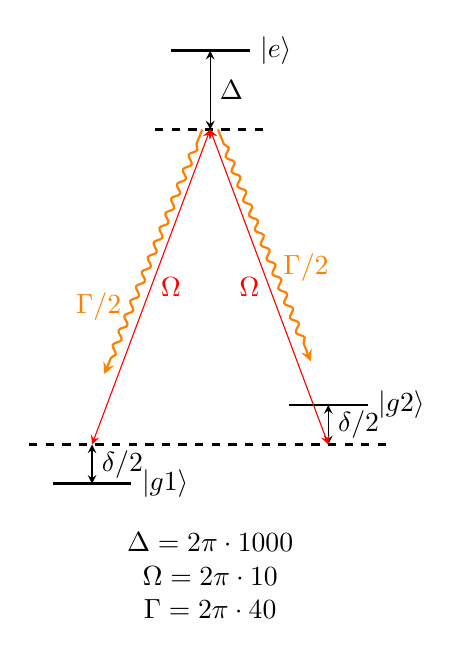
\begin{tikzpicture}
  \draw[line width=1] (0, 1) -- (1, 1) node[right] {$|e\rangle$};
  \draw[line width=1] (-1.5, -4.5) -- (-0.5, -4.5) node[right] {$|g1\rangle$};
  \draw[line width=1] (1.5, -3.5) -- (2.5, -3.5) node[right] {$|g2\rangle$};
  \draw[line width=1, dashed] (-0.2, 0) -- (1.2, 0);
  \draw[line width=1, dashed] (-1.8, -4) -- (2.8, -4);

  \draw[<->,>=stealth] (0.5, 0) -- node[right] {$\Delta$} (0.5, 1);
  \draw[<->,>=stealth] (-1, -4.5) -- node[right] {$\delta/2$} (-1, -4);
  \draw[<->,>=stealth] (2, -3.5) -- node[right] {$\delta/2$} (2, -4);

  \draw[red,<->,>=stealth] (0.5, 0) -- node[right] {$\Omega$} (-1, -4);
  \draw[red,<->,>=stealth] (0.5, 0) -- node[left] {$\Omega$} (2, -4);

  \draw[orange,->,>=stealth,decorate, decoration={pre length=0.2cm,
    post length=0.8cm, snake, amplitude=.4mm,
    segment length=2mm},thick,shorten >=0.6cm] (0.6, 0) -- node[right] {$\Gamma/2$} (2, -3.5);
  \draw[orange,->,>=stealth,decorate, decoration={pre length=0.2cm,
    post length=1.7cm, snake, amplitude=.4mm,
    segment length=2mm},thick,shorten >=1.5cm] (0.4, 0) -- node[left] {$\Gamma/2$} (-1.4, -4.5);

  \node[below,align=center] at (0.5, -5) {
    $\Delta=2\pi\cdot1000$\\
    $\Omega=2\pi\cdot10$\\
    $\Gamma=2\pi\cdot40$
  };
\end{tikzpicture}
\end{document}
